% !TEX root = ../main.tex

\section{Experimental Setup}
\label{sec:experimental-setup}

This section describes the experimental protocol used to evaluate the pipeline. The experiments are designed to assess how the extracted association rules vary across different geographical contexts, classifier architectures, and analysis configurations, with the goal of identifying robust patterns that distinguish merit-based decision logic from potentially biased behavior.

\subsection{Implementation and Execution Environment}
\label{sec:implementation-environment}

The implementation choices adopted to make the method formalized in Chapter~\ref{cap:method} executable and scalable are summarized in this subsection. The full pipeline is implemented in Python~3.10 and is organized into four sequential stages, each corresponding to an independent module. All experiments were conducted in a \texttt{conda} environment on an Apple Mac Studio platform equipped with an M1 Ultra chip, 64~GB RAM, and macOS~26.3.1\,(a) (build \texttt{25D771280a}, Darwin kernel \texttt{25.3.0}). The thesis project and all experimental runs were executed on this infrastructure at the CI\&SS Laboratory of the University of Naples ``Parthenope'' (website: \href{https://cisslab.uniparthenope.it}{cisslab.uniparthenope.it}). Additional implementation details on the software stack, parallelization strategy, and scalability considerations are reported in Appendix~\ref{app:software-stack}.

\begin{figure}[H]
\centering
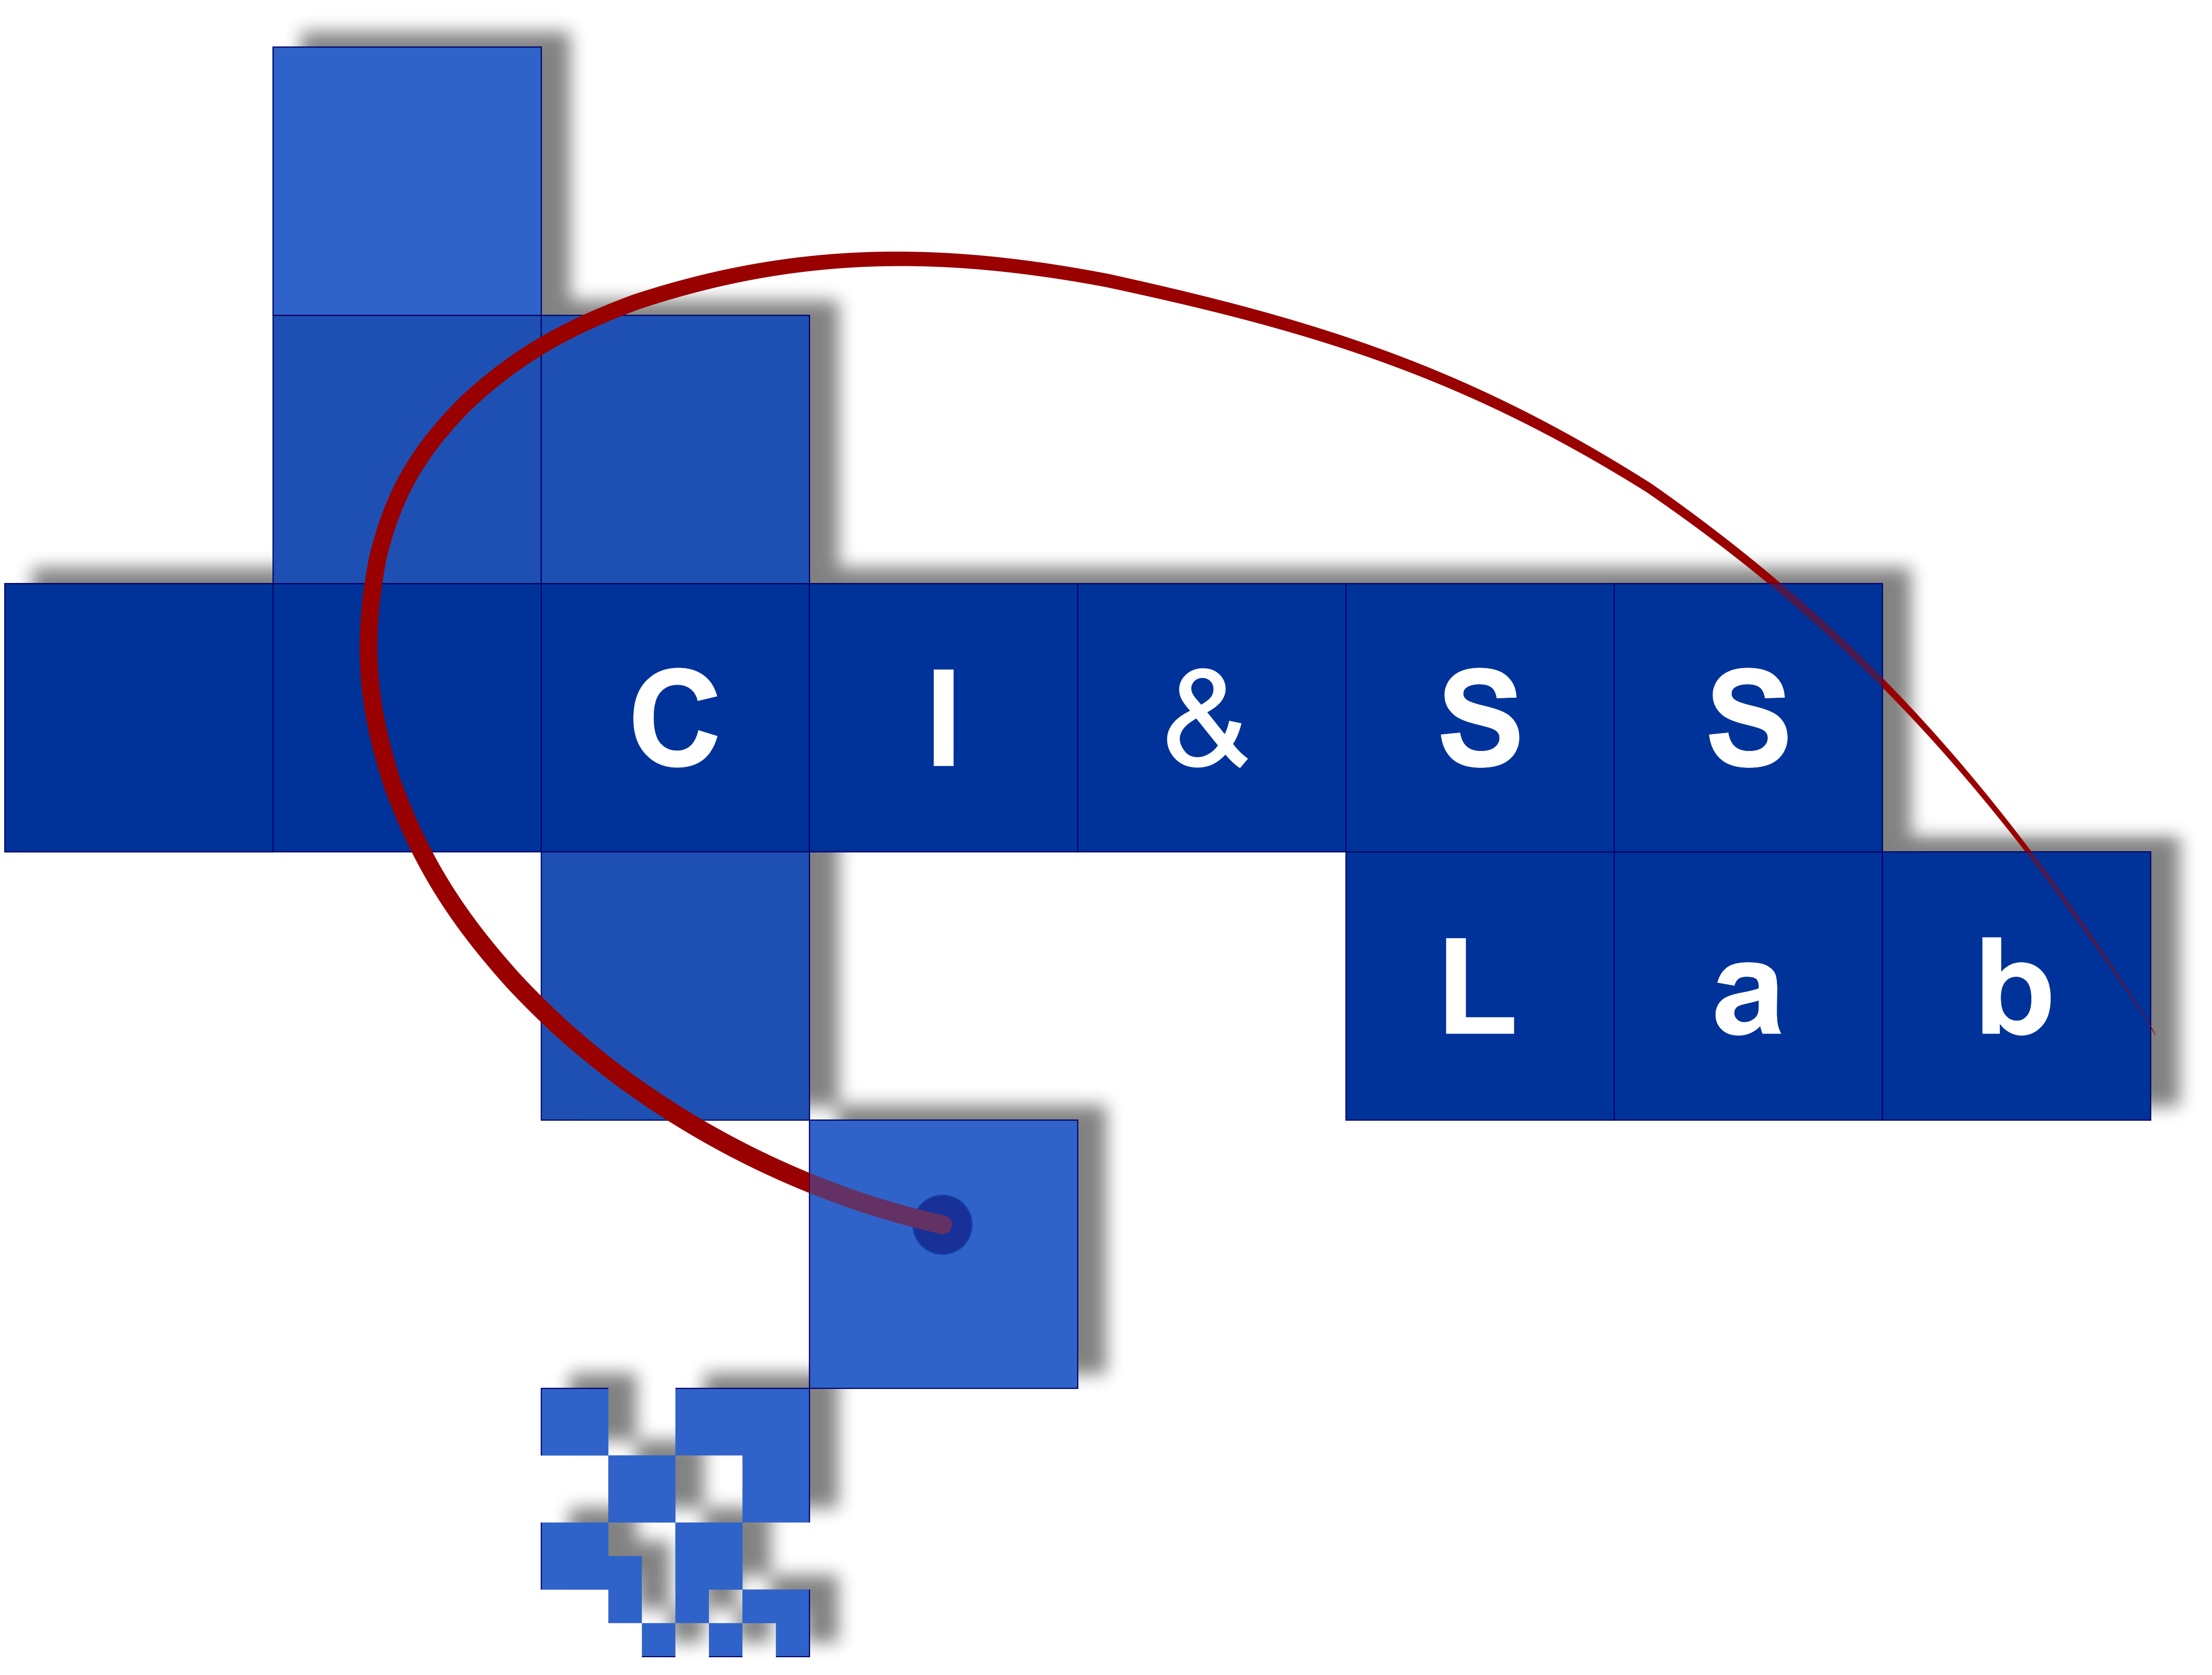
\includegraphics[width=0.32\textwidth]{assets/cisslab_logo.png}
\caption{CI\&SS Laboratory of the University of Naples ``Parthenope''.}
\label{fig:cisslab-logo}
\end{figure}

\subsection{Experiment Configurations}
\label{sec:experiment-configurations}

The pipeline was executed across multiple configurations, obtained by varying the following parameters:

\paragraph{Geographical scope.} Experiments were conducted on all five benchmark datasets described in Chapter~\ref{cap:data}: the New York metropolitan area (NY), Texas (TX), the U.S. Northeast, the U.S. South, and the set of all U.S. states except Alaska (ALL). Comparison is thereby enabled across socio-economically contrasting settings, ranging from a single metropolitan area to a national-scale dataset with over 1.4 million training instances.

\paragraph{Classifiers.} Two classifiers with fundamentally different decision boundary geometries were used: CatBoost, a gradient-boosted tree ensemble that produces axis-aligned decision splits, and MLP (Multi-Layer Perceptron), which produces smooth non-linear decision surfaces. As discussed in Chapter~\ref{cap:method}, the use of two structurally distinct classifiers allows verification that the patterns identified by the pipeline reflect properties of the data rather than artifacts of a particular model family. Since the adapted BoCSoR method is model-agnostic, patterns that emerge consistently across both classifiers carry stronger evidential weight.

\paragraph{Neighbourhood size $k$.} The number of counterfactual neighbours used in the BoCSoR analysis was varied across the set $k \in \{1, 3, 5, 7, 9, 11, 13, 15\}$. Small values of $k$ focus the analysis on the closest counterfactual neighbours, capturing the most local decision-boundary structure. Larger values broaden the neighbourhood, potentially revealing more stable and generalizable patterns at the cost of including more distant counterfactuals. By evaluating across the full range, the experiments assess the sensitivity of the extracted rules to the neighbourhood size and identify patterns that persist across multiple scales.

\paragraph{Boundary percentile $P$.} The percentile threshold for boundary instance selection was varied across $P \in \{10\%, 15\%, 20\%, 25\%\}$. This parameter controls how deep into the dataset the analysis reaches: at $P = 10\%$, only the $10\%$ of instances closest to the decision boundary are analyzed, yielding a focused but potentially sparse set of explanations. At $P = 25\%$, a broader population of near-boundary instances is included, increasing the volume of transactions available to the ARM stage but potentially diluting the signal with instances farther from the boundary. The variation of $P$ serves to assess the robustness of the extracted rules and to determine whether key patterns are stable across different boundary-proximity thresholds.

\paragraph{Overall configuration space.} The full experimental design spans 5 geographical scopes, 2 classifiers, 4 percentile values, and 8 neighbourhood sizes, yielding a total of $5 \times 2 \times 4 \times 8 = 320$ individual BoCSoR runs. Each run produces a separate transactional database, which is then independently processed by the macroscopic and microscopic ARM stages.

\subsection{Association Rule Mining Configuration}
\label{sec:arm-configuration}

The association rule mining stages operate on the transactional databases produced by BoCSoR and extract rules evaluated through three complementary metrics: support, confidence, and lift, as defined in Chapter~\ref{cap:method}.

To explore the space of possible threshold combinations systematically, the pipeline employs a grid search over support and confidence values. The support axis spans the range $[0.05, 1.00]$ and the confidence axis spans $[0.50, 1.00]$ for macroscopic rules, with step sizes automatically determined to produce approximately 40 levels per axis. For microscopic rules, the thresholds are set lower (support $\geq 0.01$, confidence $\geq 0.30$) to accommodate the smaller transaction sets that result from filtering to specific macroscopic rule anchors.

Rules whose lift falls within the interval $[0.75, 1.25]$ are discarded, as they represent near-independent co-occurrences that carry no meaningful associative information. Only rules with lift above $1.25$ (positive correlation) or below $0.75$ (negative correlation) are retained for analysis.

This grid-search approach avoids the need to commit to a single pair of thresholds \textit{a priori}. Instead, a complete landscape of rule counts is produced at each combination of support and confidence, making it possible to observe how the number of surviving rules varies as the quality bar is raised. Rules that persist at high support and high confidence thresholds are the strongest and most statistically reliable.

\subsection{Semantic Classification of Association Rules}
\label{sec:semantic-classification}

To interpret the extracted rules in the context of fairness and actionability, each rule is classified into one of three semantic categories based on the features it involves. This classification is applied to both macroscopic rules (which operate at the feature-name level, e.g., $\texttt{SCHL} \Rightarrow \texttt{OCCP}$) and microscopic rules (which operate at the feature-category level, e.g., $\texttt{SCHL=Bachelors} \Rightarrow \texttt{OCCP=Management}$).

\paragraph{Actionable rules.} A rule is classified as \emph{actionable} if \textbf{all} features appearing in both its antecedent and consequent belong exclusively to the set of actionable features: $\{\texttt{SCHL}, \texttt{COW}, \texttt{WKHP}, \texttt{OCCP}\}$. These features represent variables that a person can, at least in principle, modify through individual effort or choice: educational attainment, class of worker, weekly working hours, and occupation. Actionable rules capture the merit-based logic of the classifier, describing patterns such as ``higher education is associated with managerial occupations near the income boundary.''

\paragraph{Biased rules.} A rule is classified as \emph{biased} if it contains \textbf{at least one} sensitive feature: $\texttt{SEX}$ (sex) or $\texttt{RAC1P}$ (race). The rule may also contain any other features; the presence of even a single sensitive attribute is sufficient for classification as biased. Biased rules indicate that the classifier's decision logic, near the income boundary, is entangled with demographic attributes that should ideally be irrelevant to income prediction. A biased rule does not necessarily imply that the model is discriminatory in a legal or normative sense, but it signals that the boundary-crossing pattern involves a protected attribute and therefore warrants further scrutiny.

\paragraph{Other rules.} Rules that contain neither exclusively actionable features nor any sensitive feature are classified as \emph{other}. These typically involve contextual features such as age (\texttt{AGEP}), marital status (\texttt{MAR}), place of birth (\texttt{POBP}), or household relationship (\texttt{RELP}). While these rules contribute to the overall count and are used as the denominator for percentage calculations, they are not the primary focus of the analysis.

The classification is mutually exclusive: if a rule contains a sensitive feature, it is classified as biased regardless of whether it also contains actionable features. This conservative criterion reflects the principle that the presence of a protected attribute in the decision logic is always relevant from a fairness perspective.

At the same time, the interpretation adopted in this chapter remains deliberately descriptive and non-causal. The experimental analysis is limited to identifying, quantifying, and comparing statistical regularities in the extracted rules, namely recurring patterns of association among features near the classifier decision boundary. Consequently, terms such as \enquote{biased rules} must be understood as operational labels internal to the present analytical framework, not as definitive evidence of actual discrimination, nor as proof of an underlying sociological mechanism. Any stronger claim about real-world discriminatory phenomena, structural inequality, or the sociological meaning of the observed associations would require a separate domain-level assessment by qualified experts, such as sociologists or specialists in the application context. No such claims are made here, and no causal or normative conclusions are inferred beyond the empirical description of the patterns detected in the data and in the model behavior.

\section{Experimental Results}
\label{sec:main-results}

This section presents the main findings, organized from high-threshold baselines to detailed pattern analysis.

\subsection{High-Threshold Baseline}

At support $\geq 0.25$ and support $\geq 0.30$, no actionable or biased rules survive in any geographical scope, for either classifier, at any percentile or neighbourhood size. The only rules that persist at these thresholds involve contextual features such as age, marital status, and place of birth.

This negative result establishes the context for all subsequent findings: the merit-based and bias-related signals in the classifier's decision logic are statistically weaker than the contextual signals. They emerge only at lower support thresholds, meaning that a smaller, though still substantial, fraction of the boundary population is affected.

\subsection{Macroscopic Results at Support \texorpdfstring{$\geq 0.20$}{>= 0.20}}

At support $\geq 0.20$, the first biased rules appear. They emerge exclusively in Texas, and no actionable rules survive at this threshold in any state. Table~\ref{tab:macro-sup020} summarizes the findings.

\begin{table}[htbp]
\centering
\renewcommand{\arraystretch}{1.2}
\caption{Macroscopic rules at support $\geq 0.20$. Only configurations with at least one biased rule are shown.}
\label{tab:macro-sup020}
\begin{tabular}{>{\raggedright\arraybackslash}p{0.14\textwidth} >{\raggedright\arraybackslash}p{0.14\textwidth} p{0.08\textwidth} p{0.06\textwidth} p{0.12\textwidth} p{0.10\textwidth} p{0.10\textwidth}}
  \toprule
  \textbf{State} & \textbf{Classifier} & \textbf{Pct} & \textbf{$k$} & \textbf{Total} & \textbf{Action.} & \textbf{Biased} \\
  \midrule
  TX & CatBoost & 20 & 15 & 9 & 0 & 9 \\
  TX & MLP & 20 & 15 & 1 & 0 & 1 \\
  TX & CatBoost & 25 & 13 & 3 & 0 & 3 \\
  TX & CatBoost & 25 & 15 & 39 & 0 & 27 \\
  TX & MLP & 25 & 15 & 24 & 0 & 15 \\
  \bottomrule
\end{tabular}
\renewcommand{\arraystretch}{1.0}
\end{table}

All biased rules at this threshold share the same structural pattern: they involve race (\texttt{RAC1P}) and occupation (\texttt{OCCP}), often combined with education (\texttt{SCHL}) and age (\texttt{AGEP}). No biased rule at this threshold involves sex (\texttt{SEX}). All rules belong to class~0, i.e., they characterize the decision boundary toward lower income.

\subsection{Macroscopic Results at Support \texorpdfstring{$\geq 0.10$}{>= 0.10}}

At support $\geq 0.10$, both actionable and biased rules emerge across multiple geographical scopes, revealing a clear geographic asymmetry. Table~\ref{tab:macro-sup010} summarizes the distribution.

\begin{table}[htbp]
\centering
\renewcommand{\arraystretch}{1.2}
\caption{Macroscopic actionable and biased rules at support $\geq 0.10$, aggregated across all configurations.}
\label{tab:macro-sup010}
\begin{tabular}{>{\raggedright\arraybackslash}p{0.18\textwidth} p{0.14\textwidth} p{0.14\textwidth} p{0.38\textwidth}}
  \toprule
  \textbf{Scope} & \textbf{Actionable} & \textbf{Biased} & \textbf{Observation} \\
  \midrule
  NY & 123 & 52 & Actionable dominates ($2.4\times$) \\
  TX & 157 & 655 & Biased dominates ($4.2\times$) \\
  Northeast & 30 & 0 & Only actionable \\
  South & 28 & 102 & Biased dominates ($3.6\times$) \\
  ALL & 0 & 0 & No signal \\
  \bottomrule
\end{tabular}
\renewcommand{\arraystretch}{1.0}
\end{table}

\subsection{Macroscopic Results at Support \texorpdfstring{$\geq 0.05$}{>= 0.05}}

Lowering the support threshold to $0.05$ completes the picture. At this level, both actionable and biased rules appear in all five geographical scopes, including the national benchmark (ALL). Table~\ref{tab:macro-sup005} reports the full distribution.

\begin{table}[htbp]
\centering
\renewcommand{\arraystretch}{1.2}
\caption{Macroscopic actionable and biased rules at support $\geq 0.05$ and their ratio.}
\label{tab:macro-sup005}
\begin{tabular}{>{\raggedright\arraybackslash}p{0.18\textwidth} p{0.14\textwidth} p{0.14\textwidth} p{0.14\textwidth} p{0.24\textwidth}}
  \toprule
  \textbf{Scope} & \textbf{Actionable} & \textbf{Biased} & \textbf{Ratio} & \textbf{Observation} \\
  \midrule
  Northeast & 209 & 276 & $1.3\times$ & Nearly balanced \\
  ALL & 67 & 131 & $2.0\times$ & Mild bias prevalence \\
  NY & 303 & 796 & $2.6\times$ & Moderate bias \\
  TX & 287 & 2213 & $7.7\times$ & Strong bias \\
  South & 188 & 2213 & $11.8\times$ & Dominant bias \\
  \bottomrule
\end{tabular}
\renewcommand{\arraystretch}{1.0}
\end{table}

At this threshold, several additional findings emerge. The national benchmark (ALL) now produces 67 actionable and 131 biased rules, but these disappear already at support $\geq 0.07$, indicating that the national-level signal is real but extremely weak. The Northeast, which at support $\geq 0.10$ appeared entirely free of biased rules, now shows 276 biased rules at support $\geq 0.05$. However, these are statistically fragile: they drop to a single rule at support $\geq 0.07$ and vanish entirely at $\geq 0.10$. The Northeast may therefore be regarded as the cleanest benchmark, where any race-occupation entanglement is marginal.

The geographic asymmetry in the balance between actionable and biased rules is illustrated in Figure~\ref{fig:actionable-vs-biased}. The bias-to-actionable ratio increases monotonically from the Northeast ($1.3\times$) through the national aggregate ($2.0\times$), New York ($2.6\times$), and Texas ($7.7\times$) to the South ($11.8\times$), correlating with the socio-economic gradient described in Chapter~\ref{cap:data}.

\begin{figure}[htbp]
\centering
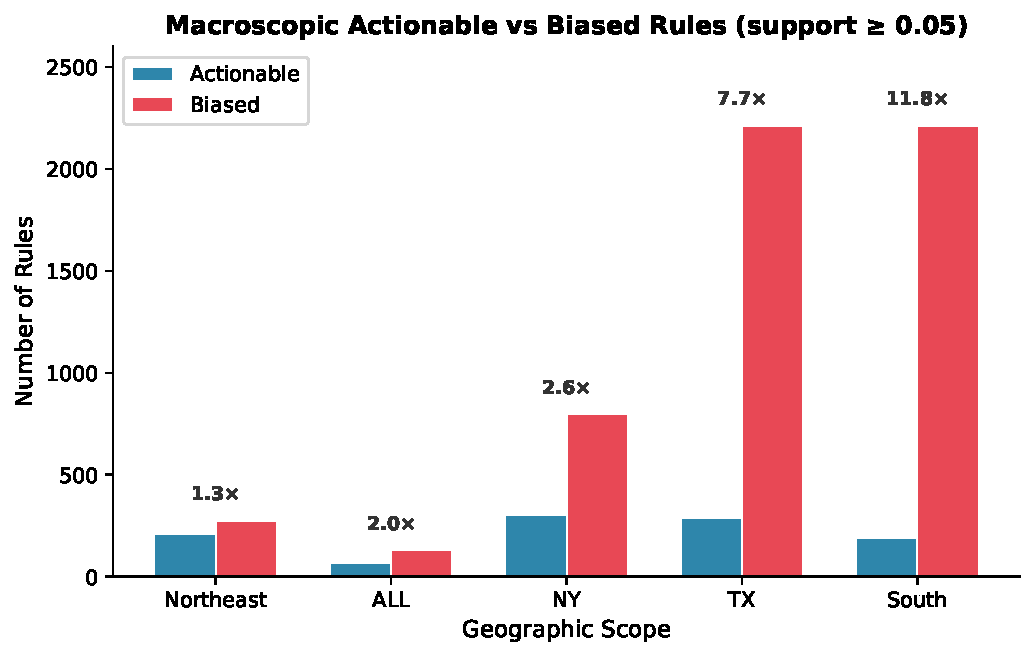
\includegraphics[width=0.85\textwidth]{assets/fig_actionable_vs_biased.pdf}
\caption{Macroscopic actionable and biased rule counts by geographic scope at support $\geq 0.05$. The bias-to-actionable ratio (annotated above each pair) increases from the more affluent benchmarks to those with higher poverty concentration.}
\label{fig:actionable-vs-biased}
\end{figure}

\subsection{Decay of Rules with Increasing Support}

Table~\ref{tab:decay} shows how actionable and biased rules disappear as the support threshold increases. This analysis reveals the relative statistical robustness of the two signals.

\begin{table}[htbp]
\centering
\renewcommand{\arraystretch}{1.2}
\caption{Actionable and biased rule counts at increasing support thresholds (summed across all configurations at the lowest confidence level).}
\label{tab:decay}
\resizebox{\textwidth}{!}{%
\begin{tabular}{>{\raggedright\arraybackslash}p{0.12\textwidth} *{5}{p{0.15\textwidth}}}
  \toprule
  \textbf{Support} & \textbf{ALL} & \textbf{NY} & \textbf{TX} & \textbf{Northeast} & \textbf{South} \\
  \midrule
  $\geq 0.05$ & 67 / 131 & 303 / 796 & 287 / 2213 & 209 / 276 & 187 / 2213 \\
  $\geq 0.07$ & 3 / 0 & 0 / 0 & 36 / 147 & 66 / 1 & 57 / 345 \\
  $\geq 0.10$ & 0 / 0 & 123 / 52 & 157 / 655 & 27 / 0 & 28 / 102 \\
  $\geq 0.15$ & 0 / 0 & 13 / 0 & 40 / 276 & 0 / 0 & 0 / 0 \\
  $\geq 0.20$ & 0 / 0 & 0 / 0 & 0 / 55 & 0 / 0 & 0 / 0 \\
  $\geq 0.25$ & 0 / 0 & 0 / 0 & 0 / 0 & 0 / 0 & 0 / 0 \\
  \bottomrule
\end{tabular}%
}
\renewcommand{\arraystretch}{1.0}
\begin{flushleft}
\small Each cell shows actionable / biased counts. NY values at support $\geq 0.07$ follow the same grid as other states.
\end{flushleft}
\end{table}

The decay patterns reveal two contrasting behaviors. In New York and the Northeast, actionable rules are more persistent than biased rules: they survive at higher support thresholds, indicating that the merit-based signal is statistically stronger than the bias signal. In Texas and the South, the opposite holds: biased rules survive up to support $\geq 0.20$ (Texas) or $\geq 0.10$ (South), while actionable rules disappear earlier. The race-occupation entanglement in these benchmarks is therefore statistically more robust than the merit-based decision patterns. Figure~\ref{fig:decay} visualizes this differential persistence.

\begin{figure}[htbp]
\centering
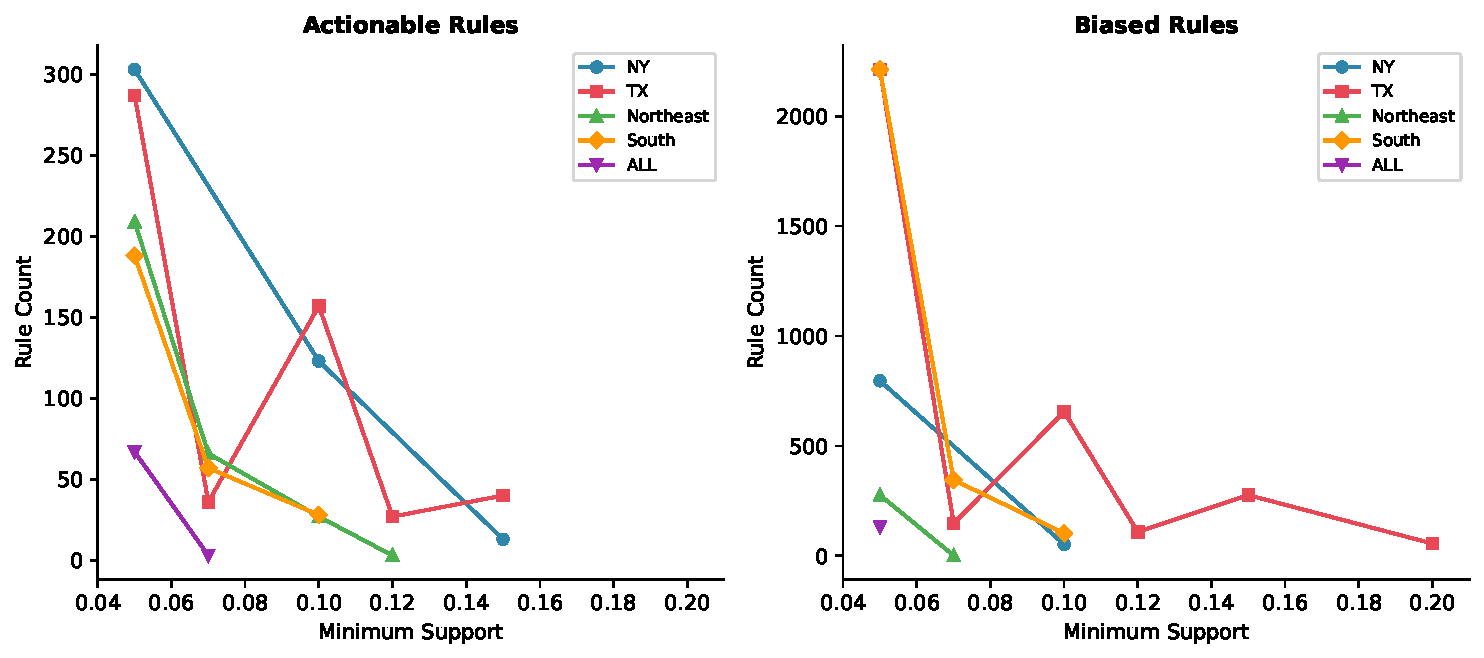
\includegraphics[width=\textwidth]{assets/fig_decay.pdf}
\caption{Decay of actionable (left) and biased (right) rules with increasing minimum support threshold. In New York and the Northeast, actionable rules persist at higher thresholds; in Texas and the South, biased rules are more robust. The ALL benchmark signal vanishes earliest.}
\label{fig:decay}
\end{figure}

\subsection{Class Asymmetry}

A consistent pattern emerges: the strong asymmetry between the two boundary directions.The vast majority of actionable and biased rules belong to class~0, which characterizes the boundary toward lower income (below the region-specific threshold $\theta$ defined in Chapter~\ref{cap:data}).

\begin{table}[htbp]
\centering
\renewcommand{\arraystretch}{1.2}
\caption{Actionable and biased rules by class direction (no support filter).}
\label{tab:class-asymmetry}
\begin{tabular}{>{\raggedright\arraybackslash}p{0.14\textwidth} p{0.18\textwidth} p{0.18\textwidth} p{0.36\textwidth}}
  \toprule
  \textbf{Class} & \textbf{Actionable} & \textbf{Biased} & \textbf{Note} \\
  \midrule
  Class 0 & 1018 & 5584 & All 5 scopes \\
  Class 1 & 36 & 45 & NY only (CatBoost and MLP) \\
  \bottomrule
\end{tabular}
\renewcommand{\arraystretch}{1.0}
\end{table}

Class~1 rules (boundary toward higher income, above $\theta$) are present only in New York, only at $k = 13$ and $k = 15$, and only at very low support ($0.05$--$0.06$). Despite their low support, these rules exhibit remarkably high lift values ($5.0$--$5.8$), indicating that the underlying patterns, while rare, are far from random. The same structural signatures observed for class~0 are also followed by class~1 rules: $\texttt{COW} \Rightarrow \texttt{OCCP}$ for actionable rules and $\texttt{RAC1P} \Rightarrow \texttt{OCCP}$ for biased rules.

This asymmetry suggests that the classifier's decision logic is more structured, and more susceptible to bias, when predicting who falls below the income threshold than when predicting who rises above it. The fact that the only exception occurs in New York, the most affluent and urbanized benchmark, is consistent with the hypothesis that class~1 patterns require a specific demographic structure to emerge.

\subsection{Dominant Macroscopic Patterns}

The actionable and biased rules that survive across multiple thresholds share distinct structural signatures. A deeper analysis of their composition reveals geographic variations in both the type of bias and the specific features involved.

\paragraph{Actionable pattern.} The dominant actionable pattern across all states is $\texttt{COW} \Rightarrow \texttt{OCCP}$ (class of worker predicts occupation), often combined with \texttt{SCHL} (education) and \texttt{WKHP} (working hours). This pattern appears in all five geographical scopes and accounts for the majority of actionable rules. The strongest individual actionable rule, observed in Texas at $k = 15$ and $P = 25\%$, achieves support $0.197$, confidence $0.857$, and lift $1.49$. In New York, the same pattern reaches higher lift values ($3.26$) but lower support ($0.174$).

\paragraph{Biased pattern: race and occupation.} The dominant biased pattern is $\texttt{RAC1P} \Rightarrow \texttt{OCCP}$ (race predicts occupation), often combined with \texttt{SCHL} and \texttt{AGEP}. This pattern appears in all five geographical scopes and is the strongest biased signal in every benchmark except the South. The strongest individual biased rule, observed in Texas, achieves support $0.236$, confidence $0.892$, and lift $1.55$. Rules involving race account for the vast majority of biased rules in every scope: $100\%$ in ALL, $77\%$ in NY, $79\%$ in TX, $67\%$ in the Northeast, and $91\%$ in the South.

\paragraph{Biased pattern: sex and occupation.} Contrary to what might be expected from the high-threshold analysis, sex (\texttt{SEX}) does appear in biased rules at support $\geq 0.05$. The pattern $\texttt{SEX} \Rightarrow \texttt{OCCP}$ emerges in four out of five scopes: NY ($186$ rules), TX ($467$), Northeast ($90$), and South ($190$). Only the ALL benchmark produces no sex-related biased rules. However, the sex signal is consistently weaker than the race signal: SEX rules have lower support (maximum $0.120$ in TX vs. $0.236$ for RAC1P) and lower lift. The Northeast shows the highest relative contribution of SEX, where $33\%$ of biased rules involve sex rather than race.

\paragraph{Geographic variation: the South and place of birth.} The South exhibits a unique biased pattern not observed as dominant in any other benchmark: $\texttt{RAC1P} \Rightarrow \texttt{POBP}$ (race predicts place of birth). This pattern accounts for $1{,}631$ out of $2{,}213$ biased rules in the South ($74\%$), making it the single most frequent biased association in that scope. By contrast, New York produces zero POBP-related biased rules, and in TX the figure is $327$ ($15\%$). This finding suggests that in the South, the classifier's decision boundary entangles race not primarily with occupation but with geographic origin, reflecting the distinct demographic structure of the region.

\paragraph{Independence of RAC1P and SEX.} The two sensitive features operate almost entirely independently in the extracted rules. Only $18$ rules out of $5{,}629$ biased rules ($0.3\%$) contain both \texttt{RAC1P} and \texttt{SEX}, and these appear exclusively in Texas. In all other scopes, no biased rule involves both sensitive attributes simultaneously. This indicates that race-related and sex-related bias, where present, follow separate structural paths in the classifier's decision logic.

The composition of biased rules by sensitive feature is illustrated in Figure~\ref{fig:bias-composition}.

\begin{figure}[htbp]
\centering
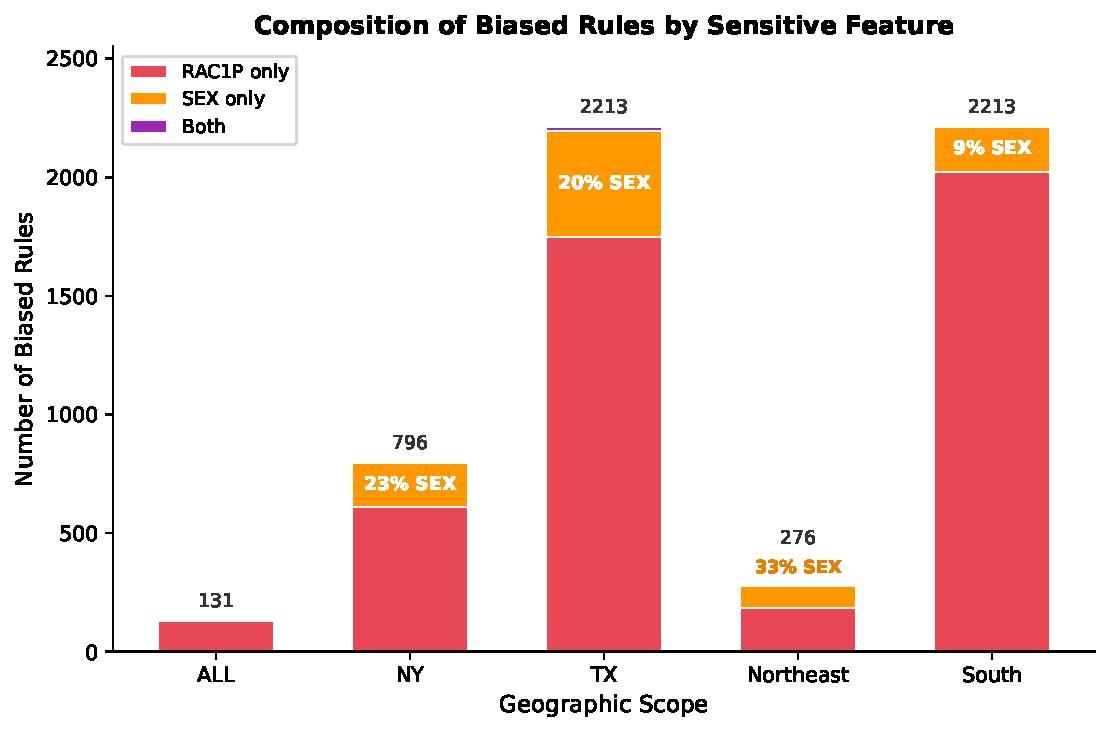
\includegraphics[width=0.85\textwidth]{assets/fig_bias_composition.pdf}
\caption{Composition of biased rules by sensitive feature across geographic scopes. Race (\texttt{RAC1P}) dominates in all benchmarks. Sex (\texttt{SEX}) contributes a secondary signal, most prominently in the Northeast ($33\%$) and New York ($23\%$). The two sensitive features almost never co-occur in the same rule.}
\label{fig:bias-composition}
\end{figure}

\subsection{Effect of Configuration Parameters}

\paragraph{Classifier comparison.} The same structural patterns are identified by both CatBoost and MLP, confirming the model-agnostic property of the pipeline. CatBoost produces more biased rules than MLP, particularly in Texas ($1150$ vs. $1063$ at support $\geq 0.05$). This is consistent with the nature of gradient-boosted trees, whose axis-aligned splits capture interactions between categorical features more readily than the smooth decision surfaces of MLP.

\paragraph{Neighbourhood size and percentile.} Larger values of $k$ (13 and 15) and higher percentiles ($20\%$ and $25\%$) produce more rules. The most informative configurations for surfacing both actionable and biased rules are $k = 15$ with $P = 25\%$. Class~1 rules appear only at $k = 13$ and $k = 15$, indicating that the higher-income boundary patterns require broader counterfactual neighbourhoods to be detected.

\paragraph{Decay with increasing support.} The differential persistence of actionable and biased rules at increasing support thresholds varies by geographic scope. In New York and the Northeast, actionable rules are more persistent; in Texas and the South, biased rules dominate. This asymmetry constitutes one of the main empirical findings documented in the thesis.

\subsection{Microscopic Results}
\label{sec:micro-results}

The macroscopic analysis identifies which features co-occur at the decision boundary; the microscopic analysis reveals the specific category values that materialize those structural dependencies. For each macroscopic rule that survives the support $\geq 0.10$ threshold, the pipeline extracts value-level rules from the filtered transaction subsets. After applying microscopic thresholds (support $\geq 0.03$, confidence $\geq 0.70$, lift $\geq 2.0$), the analysis yields $30{,}252$ actionable and $31{,}353$ biased microscopic rules. Texas dominates both categories, contributing over $99\%$ of the micro rules due to its larger volume of surviving macroscopic mothers.

\subsubsection{Microscopic Actionable Patterns}

The dominant micro-level actionable pattern across all scopes is the association between public-sector employment and the education sector. In Texas, the strongest rule is
\begin{center}
\texttt{COW=Local-Government-Employee} $\Rightarrow$ \texttt{OCCP=Educational-Instruction-And-Library}
\end{center}
with support $0.271$, confidence $0.772$, and lift $2.34$. This means that among boundary instances where class of worker and occupation are jointly relevant for the prediction, $27\%$ involve public employees in education, and $77\%$ of those who are local government employees work in educational occupations. When combined with \texttt{SCHL=Bachelors-Degree}, the confidence rises to $0.888$ and the lift to $2.89$: a bachelor's degree essentially determines the specific occupation within the public sector near the income boundary.

In New York, a different actionable profile emerges: \texttt{COW=Employee-Private-Non-Profit} $\wedge$ \texttt{OCCP=Educational-Instruction-And-Library} $\Rightarrow$ \texttt{SCHL=Masters-Degree} (confidence $0.729$, lift $5.30$). The merit-based signal in New York therefore points to private non-profit education requiring a master's degree, whereas in Texas it points to public education requiring a bachelor's.

In the South, the same structural pattern materializes: \texttt{COW=Local-Government-Employee} $\wedge$ \texttt{SCHL=Bachelors-Degree} $\Rightarrow$ \texttt{OCCP=Educational-Instruction-And-Library} (support $0.052$, lift $3.65$).

\subsubsection{Microscopic Biased Patterns}

The microscopic biased rules reveal the specific demographic profiles entangled with the classifier's decision logic.

\paragraph{Texas: gendered education sector.} Sex is the dominant sensitive feature in Texas microscopic biased rules: \texttt{SEX=Female} appears in $12{,}621$ out of $30{,}729$ biased rules ($41\%$), while \texttt{SEX=Male} appears in only $3$. The strongest gendered pattern is
\begin{center}
\texttt{COW=Local-Government-Employee} $\wedge$ \texttt{SEX=Female} $\Rightarrow$ \texttt{OCCP=Educational-Instruction-And-Library}
\end{center}
with support $0.114$ and confidence $0.787$. This reveals that the same occupation-employer pattern that drives actionable rules becomes biased when it is inseparable from the sex of the worker. In parallel, race enters through a different occupational channel: \texttt{OCCP=Office-And-Administrative-Support} $\wedge$ \texttt{SEX=Female} $\Rightarrow$ \texttt{RAC1P=Two-Or-More-Races} (support $0.073$, confidence $0.820$), and the construction sector is associated with \texttt{RAC1P=White-Alone} ($3{,}385$ rules).

\paragraph{New York: white women in office work.} In New York, the micro biased rules describe a specific demographic profile: white women (\texttt{RAC1P=White-Alone}, \texttt{SEX=Female}) in office-administrative occupations living as dependents in the household (\texttt{RELP=Biological-Son-Or-Daughter}). The highest-lift rule,
\begin{center}
\texttt{RAC1P=White-Alone} $\wedge$ \texttt{SEX=Female} $\wedge$ \texttt{WKHP=Full-Time} $\Rightarrow$ \texttt{OCCP=Office-And-Administrative} $\wedge$ \texttt{RELP=Biological-Son-Or-Daughter}
\end{center}
achieves lift $7.64$, indicating a pattern $7.6$ times more likely than expected under independence. Both sensitive features (race and sex) co-occur in $93$ out of $590$ micro biased rules, a substantially higher rate of co-occurrence than at the macroscopic level.

\paragraph{South: geographic origin and race.} Only one microscopic biased pattern survives the quality thresholds in the South:
\begin{center}
\texttt{POBP=Georgia} $\Rightarrow$ \texttt{RAC1P=Black-Or-African-American-Alone}
\end{center}
with support $0.035$, confidence $0.719$, and lift $2.27$. This is the concrete materialization of the macroscopic pattern $\texttt{RAC1P} \Rightarrow \texttt{POBP}$ that distinguishes the South from all other benchmarks: at the income boundary, being born in Georgia is strongly associated with being Black. The fact that this is the sole surviving micro biased rule in the South underscores the specificity of the regional bias signal.

\subsubsection{Summary of Microscopic Findings}

Table~\ref{tab:micro-summary} summarizes the dominant microscopic patterns by geographic scope and rule type.

\begin{table}[htbp]
\centering
\renewcommand{\arraystretch}{1.2}
\caption{Dominant microscopic patterns by scope and type. Support and lift refer to the strongest instance of each pattern.}
\label{tab:micro-summary}
\begin{tabularx}{\textwidth}{>{\raggedright\arraybackslash}p{0.10\textwidth} >{\raggedright\arraybackslash}p{0.10\textwidth} >{\raggedright\arraybackslash}X >{\centering\arraybackslash}p{0.09\textwidth} >{\centering\arraybackslash}p{0.09\textwidth} >{\centering\arraybackslash}p{0.09\textwidth}}
  \toprule
  \textbf{Scope} & \textbf{Type} & \textbf{Pattern} & \textbf{Supp.} & \textbf{Conf.} & \textbf{Lift} \\
  \midrule
  TX & Action. & Local-Govt-Employee $\Rightarrow$ Educational-Instruction & 0.271 & 0.772 & 2.34 \\
  TX & Biased & Local-Govt-Employee $\wedge$ Female $\Rightarrow$ Educational-Instruction & 0.114 & 0.787 & 3.19 \\
  TX & Biased & Office-Admin $\wedge$ Female $\Rightarrow$ Two-Or-More-Races & 0.073 & 0.820 & 2.08 \\
  NY & Action. & Non-Profit $\wedge$ Educational-Instruction $\Rightarrow$ Masters-Degree & 0.036 & 0.729 & 5.30 \\
  NY & Biased & White-Alone $\wedge$ Female $\wedge$ Full-Time $\Rightarrow$ Office-Admin $\wedge$ Biological-Child & 0.036 & 0.703 & 7.64 \\
  South & Action. & Local-Govt $\wedge$ Bachelors $\Rightarrow$ Educational-Instruction & 0.052 & 0.712 & 3.65 \\
  South & Biased & Born-Georgia $\Rightarrow$ Black-Or-African-American & 0.035 & 0.719 & 2.27 \\
  \bottomrule
\end{tabularx}
\renewcommand{\arraystretch}{1.0}
\end{table}

The microscopic analysis confirms and enriches the macroscopic findings. The structural dependency $\texttt{COW} \Rightarrow \texttt{OCCP}$ materializes as a public-education pattern in every scope where it appears. The structural dependency $\texttt{RAC1P} \Rightarrow \texttt{OCCP}$ reveals that the entanglement is not uniform across races or occupations: in Texas it involves the education sector and female workers, in New York it involves white women in office work, and in the South it takes the form of a geographic-racial association specific to the state of Georgia. These findings demonstrate that the hierarchical macro-to-micro analysis provides explanatory depth that would be inaccessible from either level alone.